\chapter{Algorithmus}
In diesem Kapitel wird der Algorithmus zur Durchführung von \ac{THB} erläutert und die Implementierung dargelegt. 

Zunächst wird die der Implementierung zu Grunde liegende Datenstruktur vorgestellt, bevor der aus zwei Phasen bestehende \ac{THB}-Algorithmus erklärt wird.

Die erste Phase des \ac{THB} besteht hauptsächlich aus der Suche nach Teilbäumen, welche unter bestimmten Voraussetzungen sich als Wurzeln für die darauf folgende zweite Phase eignet. Ausgangspunkt für diese Phase ist eine Sammlung aller Bäume, welche innerhalb des \ac{THB} bearbeitet werden sollen. 



\section{Dependency Graph als Einstiegspunkt}

\begin{quotation}
	"'\textit{Compilers also use graphs to encode the flow of values from the point where a value is created, a definition, to any point where it is used, a use. A data-dependency graph embodies this relationship} \cite{HeBIS-309344573}." 
\end{quotation}

Ein Abhängigkeitsgraph (engl.: dependency graph) stellt den Informationsfluss zwischen den Attributinstanzen eines bestimmten Parse-Baumes dar. Eine Kante von einer Attributinstanz zu einer anderen bedeutet, dass der Wert der ersten benötigt wird, um den der zweiten zu berechnen. Kanten drücken die durch die semantische Regeln auferlegten Einschrängungen aus. "'Für jeden \textit{Knoten} des Parse-Baumes, der mit dem Grammatiksymbol X bezeichnet sei, weist der Abhängigkeitsgraph für jedes mit X verbundene Attribut einen Knoten auf. Angenommen, eine mit einer Produktion p verbundene semantische Regel definiert den Wert des synthetisierten Attributes A.b durch den Wert X.c . Dann hat der Abhängigkeitsgraph eine \textit{Kante} von X.c nach A.b \cite{HeBIS-194410269}."' 

Der Algorithmus verlangt einen Abhängigkeitsgraphen, der in der ersten Phase bearbeitet wird. Zur Erstellung eines Abhängigkeitsgraphen bedarf es den Vorstufen des Compilers. Ein Scanner muss die Tokens mit Hilfe von regulären Ausdrücken einlesen und ein Parser diese in einen Parse-Baum wandeln. Aufgrund zeitlicher Begrenzung und der durch den Algorithmus gegebenen Komplexität, wird ein Abhängigkeitsgraph manuell erstellt. Dieser Ablauf wird im folgenden näher erklärt.

\subsection{Graph - Linked Implementation}\label{kap:graph} 
Ein Graph ist eine Datenstruktur, in der Informationen gespeichert werden können. Im Gegensatz zu Bäumen, die eine hierarchische Struktur besitzen, sind Graphen flexibler. Die Konsequenz daraus ist, dass Graphen auch Schleifen haben können und ein Knoten in einem Graphen nicht unbedingt erreichbar sein muss (siehe Abbildung \ref{fig:Graph}).
\begin{figure}[h]
	\centering
	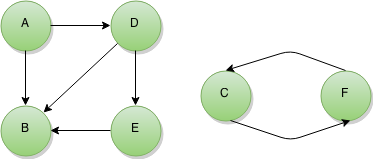
\includegraphics[scale=0.5]{images/Graph.png} 
	\caption{Beispiel eines Graphen.}
	\label{fig:Graph}
\end{figure}
Wie in Abbildung \ref{fig:Graph} zu sehen ist, besteht der Graph aus den Knoten A, B, C, D, E und F. Diese Knoten werden auch \textit{vertices} oder auch \textit{vertex} bezeichnet. Knoten \textit{können} mit einander verbunden sein. Eine Verbindung zwischen zwei Knoten wird als Kante oder auch \textit{edge} definiert und wird grafisch durch die gerichteten Pfeile dargestellt. Die Informationen sind in den jeweiligen Knoten gespeichert und werden durch die Kanten in Abhängigkeit gesetzt. 

\subsubsection*{Darstellung in C}
Ein Graph wird oft mit Hilfe einer \textit{Adjazenzmatrix\footnote{Wird auch Nachbarschaftsmatrix genannt}} oder einer \textit{Adjazenzliste} abgebildet. Eine Adjazenzmatrix ist eine 2D N x N Matrix, wobei N die Einträge der Knoten des Graphen sind. Die Matrix wird so aufgebaut, dass eine Verbindung zwischen zwei Knoten mit einer \textbf{1} versehen werden. Alle anderen Felder sind mit einer \textbf{0} gekennzeichnet. Dies hat Zufolge, dass viel Speicherplatz dadurch verbraucht wird, indem die irrelevante Information (keine Verbindung) ebenfalls dargestellt wird. Des Weiteren muss die Größe des Arrays bekannt sein. 

Abhilfe schafft hier die Adjazenzliste. Diese Liste kann mit einer "'Linked List"' in C abgebildet werden. Dabei spielt die Anzahl der Knoten keine Rolle und wird nur durch den physikalischen Speicher begrenzt. Abbildung \ref{fig:adjacencelist} zeigt den Graphen in einer Adjazenzliste. Ein Eintrag in der vertikalen Liste beinhaltet jeweils einen Knoten des Graphen und hat ein Verweis auf deren Nachfolger. Jeder Knoten speichert seine Verbindungen, also Kanten, ab. 

Eine Implementierung einer Adjazenzliste ist im Listing \ref{list:graph} abgelegt. Die vertikale Liste ist die \textit{vertex - Liste} und die horizontale Liste ist die \textit{edege - Liste}. Das Element \textit{connectTo} ist ein Pointer auf ein Vertex. Dadurch werden Kanten zwischen den Knoten definiert. Es wird also kein neuer Knoten angelegt, sondern auf einen der im Graphen enthalten ist, verwiesen. Ein Abhängigkeitsgraph speichert einen Graphen und eine Liste, der im Graphen befindlichen Variablen (UEVARS), ab.
\begin{figure}[h]
	\centering
	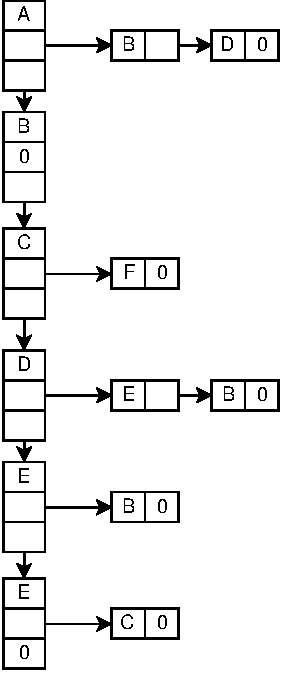
\includegraphics[scale=0.8]{images/adjacencelist.pdf} 
	\caption{Adjazenzliste des Beispiel-Graphen.}
	\label{fig:adjacencelist}
\end{figure}

\subsubsection*{Erstellung von Abhängigkeitsgraphen}
Zur Erstellung eines Abhängigkeitsgraphen werden Dateien mit der Endung "'.depg"' angelegt. Dadurch wird es Möglich eine große Anzahl von Graphen zu erstellen und den Algorithmus zu testen. Dafür wurde eine Syntax gewählt, die die Knoten, Kanten und Variablen, welche aus einem anderen Block kommen, des Graphen definieren. Dabei ist die Eingabe der Reihenfolge von Wichtigkeit, da ansonsten Zugriffsfehler entstehen können. 
Es wird verlangt, dass die Knoten zuerst definiert werden und somit die vertikale Struktur beschrieben werden kann. Dabei wird die Definition der Knoten mit \textit{vertex:} eingeleitet und mit einem Komma separiert.
Der jeweilige Knoten ist durch Brackets ("'["' , "']"') umschlossen. Hinter der Angabe des Knotennamens folgt die Definition des Knotentyps. 
\newpage
\begin{lstlisting}[caption=Struktur eines Graphen., label=list:graph]
typedef struct vertexTag {
		char* element;    
		char* operation;  
		int isConstant;
		int isVisited;
		struct edgeTag* edge;
		struct vertexTag *next;
} vertex;

typedef struct edgeTag {
		struct vertexTag *connectsTo;
		struct edgeTag *next;
} edge;

typedef struct graphTag{
		vertex *vertices;	
}graph;
\end{lstlisting}

Ähnlich werden die Verbindungen der Knoten konstruiert. Eingehend mit dem Akronym \textit{edge:} werden die Kanten mit einem Komma getrennt eingelesen. Eingeklammert in Brackets werden zwei Knoten durch einen Pfeil definiert (siehe Listing \ref{list:dg}). 

Jeder Abhängigketsgraph speichert eine Liste von Variablen, die außerhalb des Blockes definiert wurden. Das 
vorangehende \textit{uevar:} leitet eine Liste, die ebenfalls durch Kommas getrennt ist, von Variablen ein. Jede Dekleration wird mit einem Carriage return abgeschlossen.
\begin{lstlisting}[caption=Konstruktion eines Abhängigkeitsgraphen., label=list:dg]
vertex: [y(+)],[z(*)],[t1(*)],[t2(-)],[a(const)],[b(const)],[c(const)]
edge:   [y->t1] , [z->t1] , [y->t2] , [z->t2] , [t1->a] , [t1->b] ,[t2->c] 
uevar:  [a],[b],[c],[d]
\end{lstlisting}


\section{Finden von Baumkandidaten}
Zunächst werden in der ersten Phase die Baumkandidatien anhand ihrer Operation ausgewählt.

Die Operation in dem Teilbaum müssen kommutativ und assoziativ sein, sodass die Reihenfolge, in der die Operanden stehen, keinen Einfluss auf das Ergebnis haben. Beispiele für zulässige Operationen sind die Multiplikation und Addition.

Als zweites Auswahlkriterium spielt die Anzahl an Verwendungen der Teilbäume eine Rolle. Sofern ein Baum mehrfach verwendet wird, und es die mathematischen Voraussetzungen besitzt, wird es als Wurzel markiert. Bäume, die an mehreren Stellen markiert werden, sind häufig das obere Ende einer Rechnung und kommen deswegen in Frage.

Sofern der Baum einmal verwendet wird, der übergeordnete Baum jedoch eine andere Operation repräsentiert, wird er ebenfalls als Wurzel markiert. Auch in diesem Fall kann man vom oberen Ende einer Operation ausgehen.

Alle resultierenden Wurzeln werden in eine Warteschlange eingereiht, aufsteigend sortiert nach der Priorität der Operation (z.B.: Additionen niedriger priorisiert als Multiplikation).

Zu jedem Teilbaum wird innerhalb der ersten Phase der Rank auf -1 initialisiert. Dies wird in Phase 2 als zusätzliches Entscheidungskriterium für die  Unterscheidung zwischen Baum-Typen und deren Tiefe verwendet.\footnote{Die Methode \textit{NameQueue * roots(ListItem *forest)} ist im Code-Anhang unter \textit{thb/src/thb.c} zu finden.}

\section{Blockwiederherstellung in balancierter Form}
Zur Wiederherstellung der Blöcke werden drei Funktionen benutzt. In diesen wird der \ac{DG} weiter analysiert und in balancierter Form neu zusammengesetzt.

\subsection{Ausbalancieren}
Diese Funktion\footnote{Die Methode \textit{void balance(Node *root)} ist im Code-Anhang unter \textit{thb/src/thb.c} zu finden.} wird auf jeden Knoten ausgeführt, der als \textit{Root} markiert ist. Hierbei wird der Rang des Knotens festgelegt und anschließend werden die untergeordneten Knoten neu geordnet.

Zu Anfang der Funktion wird überprüft ob der aktuelle Knoten schon bearbeitet wurde. Dies kann anhand seines Rangs festgestellt werden. Initial hat ein Knoten den Rang -1. Sobald er bearbeitet wurde, wird hier ein Rang von mindestens 0 gesetzt. Wurde der Knoten noch nicht bearbeitet, wird eine neue \textit{Priority-Queue} erstellt. Diese wird an die direkt im Anschluss jeweils für den rechten und linken Teilbaum aufgerufene Funktion \textit{flatten()} durchgereicht. In ihr wird der Name und der Rang der untergeordneten Knoten, welche nicht als \textit{Root} markiert sind, gespeichert.

Der Rückgabewert der Funktion flatten() liefert den Rang. Der Rang eines als \textit{Root} markierten Knotens ist die Addition der Ränge des linken und rechten Teilbaums. Steht der Rang fest, wird der Knoten durch den Aufruf von \textit{rebuild()} neu geordnet.

\subsection{Glätten}
Diese Funktion\footnote{Die Methode \textit{int flatten(Node *var, NameQueue *q)} ist im Code-Anhang unter \textit{thb/src/thb.c} zu finden.} dient dem rekursiven durchlaufen eines Knotens und seiner Teilbäume. Initial wird sie durch die Funktion \textit{balance()} aufgerufen.\\

Diese Funktion unterscheidet in vier verschiedene Fälle:
\begin{enumerate}
	\item Beim Knoten handelt es sich um eine Konstante:\\
	Der Rang wird auf 0 gesetzt und der Knoten wird der \textit{Priority-Queue} hinzugefügt.
	\item Der Knoten ist in UEVar vorhanden:\\
	In UEvar sind alle Elemente gespeichert die von einem übergeordneten Knoten kommen. Ist dies der Fall wird der Rang auf 1 gesetzt und der Knoten wird der \textit{Priority-Queue} hinzugefügt.
	\item Der Knoten ist als \textit{Root} markiert:\\
	In diesem Fall wird die Funktion \textit{balance()} mit dem aktuellen Knoten als Parameter aufgerufen. Hierdurch wird eine neue \textit{Priority-Queue} angelegt und die untergeordneten Knoten werden weiter optimiert. Anschließend wird auch dieser Knoten der bereits vorhandenen \textit{Priority-Queue} hinzugefügt.
	\item Alle anderen Fälle:\\
	Für den jeweils linken und rechten Teilbaum wird die Funktion \textit{flatten()} aufgerufen um rekursiv bis an das Ende des Baums zu gelangen.
\end{enumerate}

Wurden alle Knoten so durchlaufen kann mit Hilfe der Funktion \textit{rebuild()} der optimierte Baum aufgebaut werden.

\subsection{Baumwiederherstellung}

Bei der letzten Phase des \ac{THB}-Algorithmus handelt es sich um das Wiederherstellen der Bäume aus den vorherigen Verarbeitungsschritten.

Hierbei muss die verarbeitende Methode\footnote{Die Methode \textit{void rebuild(NameQueue *q, Operation *op)} ist im Code-Anhang unter \textit{thb/src/thb.c} zu finden.} folgende Schritte vollführen:

Als Parameter erhält die Methode eine Liste mit Namen sowie den zugehörigen Operator - wie eingangs erwähnt, muss dieser für den kompletten Teilbaum gleich sein. Es werden nun die beiden obersten Elemente aus der Liste entnommen (diese sind nach Rang sortiert, also werden immer die Elemente mit dem niedrigsten Rang entnommen) und mit diesen ein neuer Knoten erstellt.

Handelt es sich bei beiden Elementen um Variablen, werden die Knoten mit dem zugehörigen Operator gefaltet und entweder als Wurzel gesetzt (wenn die Liste leer ist) oder als neuer Knoten wieder in die Liste eingereiht.

Ist wenigstens einer der beiden Knoten keine Variable, wird zunächst erneut der Status der Liste abgefragt. Ist diese leer, ist der Algorithmus beim Wurzelknoten angekommen und der Baum, der nun an diesem Knoten hängt, kann in die Liste der Ergebnisbäume eingetragen werden.

Ist die Liste nicht leer, wird eine neue temporäre Variable für den neuen Knoten erstellt und dieser in die Liste eingereiht. Der Rang ergibt sich hierbei in jedem Fall aus der Summe der Ränge der beiden Kindknoten, die eingangs aus der Liste extrahiert wurden.

Der hier verwendete Algorithmus geht so vor, dass die innerhalb der Schleife entstehenden Teilbäume zunächst in eine Liste eingetragen werden, aus der im Anschluss mittels der Methode \textit{Tree *getTreeFromList(ListItem *list)} der fertige Baum generiert wird. Die aus jedem Aufruf der \textit{rebuild}-Methode entstandenen Bäume werden in der globalen Variable \textit{resultTrees} gespeichert.